\documentclass[twoside]{book}

% Packages required by doxygen
\usepackage{fixltx2e}
\usepackage{calc}
\usepackage{doxygen}
\usepackage[export]{adjustbox} % also loads graphicx
\usepackage{graphicx}
\usepackage[utf8]{inputenc}
\usepackage{makeidx}
\usepackage{multicol}
\usepackage{multirow}
\PassOptionsToPackage{warn}{textcomp}
\usepackage{textcomp}
\usepackage[nointegrals]{wasysym}
\usepackage[table]{xcolor}

% Font selection
\usepackage[T1]{fontenc}
\usepackage[scaled=.90]{helvet}
\usepackage{courier}
\usepackage{amssymb}
\usepackage{sectsty}
\renewcommand{\familydefault}{\sfdefault}
\allsectionsfont{%
  \fontseries{bc}\selectfont%
  \color{darkgray}%
}
\renewcommand{\DoxyLabelFont}{%
  \fontseries{bc}\selectfont%
  \color{darkgray}%
}
\newcommand{\+}{\discretionary{\mbox{\scriptsize$\hookleftarrow$}}{}{}}

% Page & text layout
\usepackage{geometry}
\geometry{%
  a4paper,%
  top=2.5cm,%
  bottom=2.5cm,%
  left=2.5cm,%
  right=2.5cm%
}
\tolerance=750
\hfuzz=15pt
\hbadness=750
\setlength{\emergencystretch}{15pt}
\setlength{\parindent}{0cm}
\setlength{\parskip}{0.2cm}
\makeatletter
\renewcommand{\paragraph}{%
  \@startsection{paragraph}{4}{0ex}{-1.0ex}{1.0ex}{%
    \normalfont\normalsize\bfseries\SS@parafont%
  }%
}
\renewcommand{\subparagraph}{%
  \@startsection{subparagraph}{5}{0ex}{-1.0ex}{1.0ex}{%
    \normalfont\normalsize\bfseries\SS@subparafont%
  }%
}
\makeatother

% Headers & footers
\usepackage{fancyhdr}
\pagestyle{fancyplain}
\fancyhead[LE]{\fancyplain{}{\bfseries\thepage}}
\fancyhead[CE]{\fancyplain{}{}}
\fancyhead[RE]{\fancyplain{}{\bfseries\leftmark}}
\fancyhead[LO]{\fancyplain{}{\bfseries\rightmark}}
\fancyhead[CO]{\fancyplain{}{}}
\fancyhead[RO]{\fancyplain{}{\bfseries\thepage}}
\fancyfoot[LE]{\fancyplain{}{}}
\fancyfoot[CE]{\fancyplain{}{}}
\fancyfoot[RE]{\fancyplain{}{\bfseries\scriptsize Generated on Sat Nov 28 2015 22\+:59\+:50 for Pacman by Doxygen }}
\fancyfoot[LO]{\fancyplain{}{\bfseries\scriptsize Generated on Sat Nov 28 2015 22\+:59\+:50 for Pacman by Doxygen }}
\fancyfoot[CO]{\fancyplain{}{}}
\fancyfoot[RO]{\fancyplain{}{}}
\renewcommand{\footrulewidth}{0.4pt}
\renewcommand{\chaptermark}[1]{%
  \markboth{#1}{}%
}
\renewcommand{\sectionmark}[1]{%
  \markright{\thesection\ #1}%
}

% Indices & bibliography
\usepackage{natbib}
\usepackage[titles]{tocloft}
\setcounter{tocdepth}{3}
\setcounter{secnumdepth}{5}
\makeindex

% Hyperlinks (required, but should be loaded last)
\usepackage{ifpdf}
\ifpdf
  \usepackage[pdftex,pagebackref=true]{hyperref}
\else
  \usepackage[ps2pdf,pagebackref=true]{hyperref}
\fi
\hypersetup{%
  colorlinks=true,%
  linkcolor=blue,%
  citecolor=blue,%
  unicode%
}

% Custom commands
\newcommand{\clearemptydoublepage}{%
  \newpage{\pagestyle{empty}\cleardoublepage}%
}


%===== C O N T E N T S =====

\begin{document}

% Titlepage & ToC
\hypersetup{pageanchor=false,
             bookmarks=true,
             bookmarksnumbered=true,
             pdfencoding=unicode
            }
\pagenumbering{roman}
\begin{titlepage}
\vspace*{7cm}
\begin{center}%
{\Large Pacman \\[1ex]\large 0.\+5 }\\
\vspace*{1cm}
{\large Generated by Doxygen 1.8.10}\\
\vspace*{0.5cm}
{\small Sat Nov 28 2015 22:59:50}\\
\end{center}
\end{titlepage}
\clearemptydoublepage
\tableofcontents
\clearemptydoublepage
\pagenumbering{arabic}
\hypersetup{pageanchor=true}

%--- Begin generated contents ---
\chapter{Pacman}
\label{md__c_1__users_kelku__documents__git_hub_pac__pacman__r_e_a_d_m_e}
\hypertarget{md__c_1__users_kelku__documents__git_hub_pac__pacman__r_e_a_d_m_e}{}
Projet de Génie Logiciel du M1 informatique de St Jerôme \+: création du jeu \hyperlink{class_pacman}{Pacman}. 
\chapter{Hierarchical Index}
\section{Class Hierarchy}
This inheritance list is sorted roughly, but not completely, alphabetically\+:\begin{DoxyCompactList}
\item \contentsline{section}{Bille\+Array}{\pageref{class_bille_array}}{}
\item \contentsline{section}{Bonus}{\pageref{class_bonus}}{}
\begin{DoxyCompactList}
\item \contentsline{section}{Bille}{\pageref{class_bille}}{}
\item \contentsline{section}{Fruit}{\pageref{class_fruit}}{}
\end{DoxyCompactList}
\item \contentsline{section}{Collisions}{\pageref{class_collisions}}{}
\item \contentsline{section}{Labyrinthe}{\pageref{class_labyrinthe}}{}
\item \contentsline{section}{Personnage}{\pageref{class_personnage}}{}
\begin{DoxyCompactList}
\item \contentsline{section}{Fantome}{\pageref{class_fantome}}{}
\item \contentsline{section}{Pacman}{\pageref{class_pacman}}{}
\end{DoxyCompactList}
\item \contentsline{section}{Porte}{\pageref{class_porte}}{}
\item Q\+Main\+Window\begin{DoxyCompactList}
\item \contentsline{section}{Main\+Window}{\pageref{class_main_window}}{}
\end{DoxyCompactList}
\item Q\+Object\begin{DoxyCompactList}
\item \contentsline{section}{Affichage}{\pageref{class_affichage}}{}
\end{DoxyCompactList}
\item \contentsline{section}{Sound}{\pageref{class_sound}}{}
\end{DoxyCompactList}

\chapter{Class Index}
\section{Class List}
Here are the classes, structs, unions and interfaces with brief descriptions\+:\begin{DoxyCompactList}
\item\contentsline{section}{\hyperlink{class_affichage}{Affichage} }{\pageref{class_affichage}}{}
\item\contentsline{section}{\hyperlink{class_bille}{Bille} }{\pageref{class_bille}}{}
\item\contentsline{section}{\hyperlink{class_bille_array}{Bille\+Array} }{\pageref{class_bille_array}}{}
\item\contentsline{section}{\hyperlink{class_bonus}{Bonus} }{\pageref{class_bonus}}{}
\item\contentsline{section}{\hyperlink{class_collisions}{Collisions} }{\pageref{class_collisions}}{}
\item\contentsline{section}{\hyperlink{class_fantome}{Fantome} }{\pageref{class_fantome}}{}
\item\contentsline{section}{\hyperlink{class_fruit}{Fruit} }{\pageref{class_fruit}}{}
\item\contentsline{section}{\hyperlink{class_labyrinthe}{Labyrinthe} }{\pageref{class_labyrinthe}}{}
\item\contentsline{section}{\hyperlink{class_main_window}{Main\+Window} }{\pageref{class_main_window}}{}
\item\contentsline{section}{\hyperlink{class_pacman}{Pacman} }{\pageref{class_pacman}}{}
\item\contentsline{section}{\hyperlink{class_personnage}{Personnage} }{\pageref{class_personnage}}{}
\item\contentsline{section}{\hyperlink{class_porte}{Porte} }{\pageref{class_porte}}{}
\item\contentsline{section}{\hyperlink{class_sound}{Sound} }{\pageref{class_sound}}{}
\end{DoxyCompactList}

\chapter{Class Documentation}
\hypertarget{class_collisions}{}\section{Collisions Class Reference}
\label{class_collisions}\index{Collisions@{Collisions}}
\subsection*{Public Member Functions}
\begin{DoxyCompactItemize}
\item 
\hypertarget{class_collisions_a006630da4b62b10ebf123c6333c2b198}{}\hyperlink{class_collisions_a006630da4b62b10ebf123c6333c2b198}{Collisions} ()\label{class_collisions_a006630da4b62b10ebf123c6333c2b198}

\begin{DoxyCompactList}\small\item\em \hyperlink{class_collisions_a006630da4b62b10ebf123c6333c2b198}{Collisions\+::\+Collisions} constructeur par défaut. \end{DoxyCompactList}\item 
bool \hyperlink{class_collisions_a121f130f16ab50d0c7374028137dd984}{colliding} (\hyperlink{class_pacman}{Pacman} $\ast$obj1, \hyperlink{class_fantome}{Fantome} $\ast$obj2)
\begin{DoxyCompactList}\small\item\em \hyperlink{class_collisions_a121f130f16ab50d0c7374028137dd984}{Collisions\+::colliding} collision entre \hyperlink{class_pacman}{Pacman} et les fantomes. \end{DoxyCompactList}\item 
int \hyperlink{class_collisions_abb2c6a1d9521cf58911f212e2817dfc7}{colliding} (\hyperlink{class_pacman}{Pacman} $\ast$obj1, \hyperlink{class_bille_array}{Bille\+Array} $\ast$obj2)
\begin{DoxyCompactList}\small\item\em \hyperlink{class_collisions_a121f130f16ab50d0c7374028137dd984}{Collisions\+::colliding} Collision entre pacman et les croquettes. \end{DoxyCompactList}\item 
bool \hyperlink{class_collisions_adabbc973e6cb6880f93b338538f05efa}{colliding} (\hyperlink{class_pacman}{Pacman} $\ast$obj1, \hyperlink{class_fruit}{Fruit} $\ast$obj2)
\begin{DoxyCompactList}\small\item\em \hyperlink{class_collisions_a121f130f16ab50d0c7374028137dd984}{Collisions\+::colliding} Collision entre \hyperlink{class_pacman}{Pacman} et un fruit. \end{DoxyCompactList}\item 
\hypertarget{class_collisions_a5c22844d08ebf198357076dbe0d64966}{}void {\bfseries colliding} (\hyperlink{class_personnage}{Personnage} $\ast$obj1, \hyperlink{class_labyrinthe}{Labyrinthe} $\ast$obj2)\label{class_collisions_a5c22844d08ebf198357076dbe0d64966}

\item 
\hypertarget{class_collisions_a0921b974606f241b29da427dc26b2716}{}void {\bfseries colliding} (\hyperlink{class_pacman}{Pacman} $\ast$obj1, \hyperlink{class_porte}{Porte} $\ast$obj2)\label{class_collisions_a0921b974606f241b29da427dc26b2716}

\item 
\hypertarget{class_collisions_ad2f30075fe874c81a1eb6912dcab6932}{}bool {\bfseries colliding} (\hyperlink{class_fantome}{Fantome} $\ast$obj1, \hyperlink{class_porte}{Porte} $\ast$obj2)\label{class_collisions_ad2f30075fe874c81a1eb6912dcab6932}

\end{DoxyCompactItemize}


\subsection{Member Function Documentation}
\hypertarget{class_collisions_a121f130f16ab50d0c7374028137dd984}{}\index{Collisions@{Collisions}!colliding@{colliding}}
\index{colliding@{colliding}!Collisions@{Collisions}}
\subsubsection[{colliding(\+Pacman $\ast$obj1, Fantome $\ast$obj2)}]{\setlength{\rightskip}{0pt plus 5cm}bool Collisions\+::colliding (
\begin{DoxyParamCaption}
\item[{{\bf Pacman} $\ast$}]{obj1, }
\item[{{\bf Fantome} $\ast$}]{obj2}
\end{DoxyParamCaption}
)}\label{class_collisions_a121f130f16ab50d0c7374028137dd984}


\hyperlink{class_collisions_a121f130f16ab50d0c7374028137dd984}{Collisions\+::colliding} collision entre \hyperlink{class_pacman}{Pacman} et les fantomes. 


\begin{DoxyParams}{Parameters}
{\em obj1} & pointer vers \hyperlink{class_pacman}{Pacman} \\
\hline
{\em obj2} & pointer vers Fantôme \\
\hline
\end{DoxyParams}
\begin{DoxyReturn}{Returns}
Vrai si collision, faux sinon 
\end{DoxyReturn}
\hypertarget{class_collisions_abb2c6a1d9521cf58911f212e2817dfc7}{}\index{Collisions@{Collisions}!colliding@{colliding}}
\index{colliding@{colliding}!Collisions@{Collisions}}
\subsubsection[{colliding(\+Pacman $\ast$obj1, Bille\+Array $\ast$obj2)}]{\setlength{\rightskip}{0pt plus 5cm}int Collisions\+::colliding (
\begin{DoxyParamCaption}
\item[{{\bf Pacman} $\ast$}]{obj1, }
\item[{{\bf Bille\+Array} $\ast$}]{obj2}
\end{DoxyParamCaption}
)}\label{class_collisions_abb2c6a1d9521cf58911f212e2817dfc7}


\hyperlink{class_collisions_a121f130f16ab50d0c7374028137dd984}{Collisions\+::colliding} Collision entre pacman et les croquettes. 


\begin{DoxyParams}{Parameters}
{\em obj1} & pointer vers \hyperlink{class_pacman}{Pacman} \\
\hline
{\em obj2} & pointer vers Croquette \\
\hline
\end{DoxyParams}
\begin{DoxyReturn}{Returns}
retourne le numéro de la bille avec laquelle il y a collision sinon 
\end{DoxyReturn}
\hypertarget{class_collisions_adabbc973e6cb6880f93b338538f05efa}{}\index{Collisions@{Collisions}!colliding@{colliding}}
\index{colliding@{colliding}!Collisions@{Collisions}}
\subsubsection[{colliding(\+Pacman $\ast$obj1, Fruit $\ast$obj2)}]{\setlength{\rightskip}{0pt plus 5cm}bool Collisions\+::colliding (
\begin{DoxyParamCaption}
\item[{{\bf Pacman} $\ast$}]{obj1, }
\item[{{\bf Fruit} $\ast$}]{obj2}
\end{DoxyParamCaption}
)}\label{class_collisions_adabbc973e6cb6880f93b338538f05efa}


\hyperlink{class_collisions_a121f130f16ab50d0c7374028137dd984}{Collisions\+::colliding} Collision entre \hyperlink{class_pacman}{Pacman} et un fruit. 


\begin{DoxyParams}{Parameters}
{\em obj1} & \\
\hline
{\em obj2} & \\
\hline
\end{DoxyParams}
\begin{DoxyReturn}{Returns}

\end{DoxyReturn}


The documentation for this class was generated from the following files\+:\begin{DoxyCompactItemize}
\item 
C\+:/\+Users/kelku/\+Documents/\+Git\+Hub/pac/\+Pacman/collisions.\+h\item 
C\+:/\+Users/kelku/\+Documents/\+Git\+Hub/pac/\+Pacman/collisions.\+cpp\end{DoxyCompactItemize}

\hypertarget{class_fantome}{}\section{Fantome Class Reference}
\label{class_fantome}\index{Fantome@{Fantome}}


Inheritance diagram for Fantome\+:

\hypertarget{class_labyrinthe}{}\section{Labyrinthe Class Reference}
\label{class_labyrinthe}\index{Labyrinthe@{Labyrinthe}}
\subsection*{Public Member Functions}
\begin{DoxyCompactItemize}
\item 
\hypertarget{class_labyrinthe_a5ee4a2803de1dca1116c7e6c8f08b5d0}{}{\bfseries Labyrinthe} (float, float, int, int)\label{class_labyrinthe_a5ee4a2803de1dca1116c7e6c8f08b5d0}

\item 
\hypertarget{class_labyrinthe_aade17610e33994e5e021684915529db4}{}int {\bfseries get\+X} ()\label{class_labyrinthe_aade17610e33994e5e021684915529db4}

\item 
\hypertarget{class_labyrinthe_af78626c211db2bdb5b63ad6970051d4f}{}int {\bfseries get\+Y} ()\label{class_labyrinthe_af78626c211db2bdb5b63ad6970051d4f}

\end{DoxyCompactItemize}


The documentation for this class was generated from the following file\+:\begin{DoxyCompactItemize}
\item 
C\+:/\+Users/kelku/\+Documents/\+Git\+Hub/pac/\+Pacman/labyrinthe.\+h\end{DoxyCompactItemize}

\hypertarget{class_main_window}{}\section{Main\+Window Class Reference}
\label{class_main_window}\index{Main\+Window@{Main\+Window}}
Inheritance diagram for Main\+Window\+:\begin{figure}[H]
\begin{center}
\leavevmode
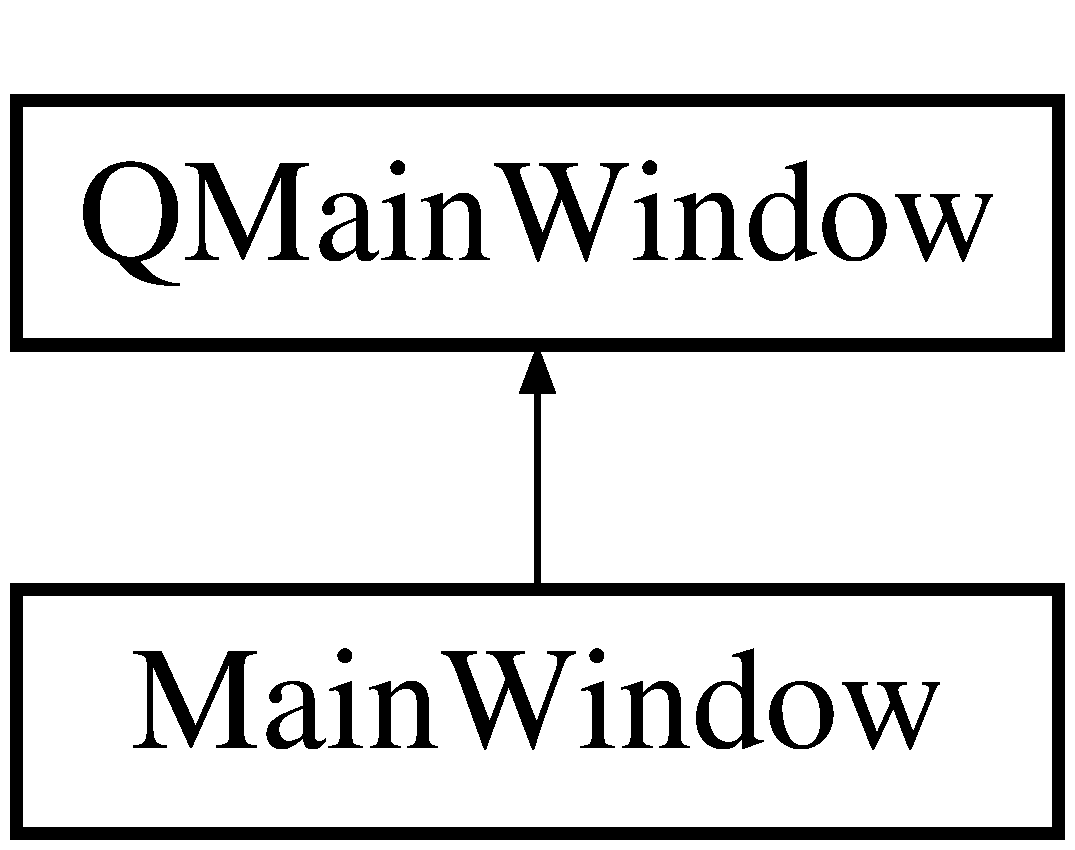
\includegraphics[height=2.000000cm]{class_main_window}
\end{center}
\end{figure}
\subsection*{Public Slots}
\begin{DoxyCompactItemize}
\item 
\hypertarget{class_main_window_a48965b8c40edf53d61e2d41977c1566d}{}void \hyperlink{class_main_window_a48965b8c40edf53d61e2d41977c1566d}{tick} ()\label{class_main_window_a48965b8c40edf53d61e2d41977c1566d}

\begin{DoxyCompactList}\small\item\em \hyperlink{class_main_window_a48965b8c40edf53d61e2d41977c1566d}{Main\+Window\+::tick} vérifie si il y a collision entre les différentes entités du jeu. \end{DoxyCompactList}\end{DoxyCompactItemize}
\subsection*{Public Member Functions}
\begin{DoxyCompactItemize}
\item 
\hypertarget{class_main_window_a8b244be8b7b7db1b08de2a2acb9409db}{}{\bfseries Main\+Window} (Q\+Widget $\ast$parent=0)\label{class_main_window_a8b244be8b7b7db1b08de2a2acb9409db}

\item 
\hypertarget{class_main_window_a2e0ce6e999817f456b6d94adf80b8faf}{}void \hyperlink{class_main_window_a2e0ce6e999817f456b6d94adf80b8faf}{show\+Event} (Q\+Show\+Event $\ast$)\label{class_main_window_a2e0ce6e999817f456b6d94adf80b8faf}

\begin{DoxyCompactList}\small\item\em \hyperlink{class_main_window_a2e0ce6e999817f456b6d94adf80b8faf}{Main\+Window\+::show\+Event} Fabrique la scence en y incluant le labyrinthe, et les différentes entités qui vont y être. \end{DoxyCompactList}\item 
\hypertarget{class_main_window_a8851a931482834eeec527490eedaf20e}{}void \hyperlink{class_main_window_a8851a931482834eeec527490eedaf20e}{resize\+Event} (Q\+Resize\+Event $\ast$)\label{class_main_window_a8851a931482834eeec527490eedaf20e}

\begin{DoxyCompactList}\small\item\em \hyperlink{class_main_window_a8851a931482834eeec527490eedaf20e}{Main\+Window\+::resize\+Event} Permet de modifier la taille des éléments lors d\textquotesingle{}un changement de la taille de la fenêtre. \end{DoxyCompactList}\item 
void \hyperlink{class_main_window_a6b8e934fca603cf7678eabb9a6dfc709}{key\+Press\+Event} (Q\+Key\+Event $\ast$)
\begin{DoxyCompactList}\small\item\em \hyperlink{class_main_window_a6b8e934fca603cf7678eabb9a6dfc709}{Main\+Window\+::key\+Press\+Event} Permet de gérer les évennement en fonction de la touche enfoncé sur le clavier. \end{DoxyCompactList}\item 
\hypertarget{class_main_window_a849e207918b12307f9cd0a576076946b}{}void {\bfseries mouse\+Press\+Event} (Q\+Mouse\+Event $\ast$)\label{class_main_window_a849e207918b12307f9cd0a576076946b}

\item 
void \hyperlink{class_main_window_aa626dd9c66b3231ec5d8f123e991af1b}{move\+Ghost} (Q\+Key\+Event $\ast$e, Fantome\+::name N)
\begin{DoxyCompactList}\small\item\em \hyperlink{class_main_window_aa626dd9c66b3231ec5d8f123e991af1b}{Main\+Window\+::move\+Ghost} Permet de gérer le déplacement des fantômes. \end{DoxyCompactList}\end{DoxyCompactItemize}


\subsection{Member Function Documentation}
\hypertarget{class_main_window_a6b8e934fca603cf7678eabb9a6dfc709}{}\index{Main\+Window@{Main\+Window}!key\+Press\+Event@{key\+Press\+Event}}
\index{key\+Press\+Event@{key\+Press\+Event}!Main\+Window@{Main\+Window}}
\subsubsection[{key\+Press\+Event(\+Q\+Key\+Event $\ast$)}]{\setlength{\rightskip}{0pt plus 5cm}void Main\+Window\+::key\+Press\+Event (
\begin{DoxyParamCaption}
\item[{Q\+Key\+Event $\ast$}]{e}
\end{DoxyParamCaption}
)}\label{class_main_window_a6b8e934fca603cf7678eabb9a6dfc709}


\hyperlink{class_main_window_a6b8e934fca603cf7678eabb9a6dfc709}{Main\+Window\+::key\+Press\+Event} Permet de gérer les évennement en fonction de la touche enfoncé sur le clavier. 


\begin{DoxyParams}{Parameters}
{\em e} & touche appuyé \\
\hline
\end{DoxyParams}
\hypertarget{class_main_window_aa626dd9c66b3231ec5d8f123e991af1b}{}\index{Main\+Window@{Main\+Window}!move\+Ghost@{move\+Ghost}}
\index{move\+Ghost@{move\+Ghost}!Main\+Window@{Main\+Window}}
\subsubsection[{move\+Ghost(\+Q\+Key\+Event $\ast$e, Fantome\+::name N)}]{\setlength{\rightskip}{0pt plus 5cm}void Main\+Window\+::move\+Ghost (
\begin{DoxyParamCaption}
\item[{Q\+Key\+Event $\ast$}]{e, }
\item[{Fantome\+::name}]{N}
\end{DoxyParamCaption}
)}\label{class_main_window_aa626dd9c66b3231ec5d8f123e991af1b}


\hyperlink{class_main_window_aa626dd9c66b3231ec5d8f123e991af1b}{Main\+Window\+::move\+Ghost} Permet de gérer le déplacement des fantômes. 


\begin{DoxyParams}{Parameters}
{\em e} & touche appuyé \\
\hline
{\em N} & fantôme sélectionné \\
\hline
\end{DoxyParams}


The documentation for this class was generated from the following files\+:\begin{DoxyCompactItemize}
\item 
C\+:/\+Users/kelku/\+Documents/\+Git\+Hub/pac/\+Pacman/mainwindow.\+h\item 
C\+:/\+Users/kelku/\+Documents/\+Git\+Hub/pac/\+Pacman/mainwindow.\+cpp\end{DoxyCompactItemize}

\hypertarget{class_pacman}{}\section{Pacman Class Reference}
\label{class_pacman}\index{Pacman@{Pacman}}


Inheritance diagram for Pacman\+:
% FIG 0


Collaboration diagram for Pacman\+:
% FIG 1
\subsection*{Public Member Functions}
\begin{DoxyCompactItemize}
\item 
\hypertarget{class_pacman_a499408baab38f119ebd4f41e90fbe3fe}{}\hyperlink{class_pacman_a499408baab38f119ebd4f41e90fbe3fe}{Pacman} ()\label{class_pacman_a499408baab38f119ebd4f41e90fbe3fe}

\begin{DoxyCompactList}\small\item\em \hyperlink{class_pacman_a499408baab38f119ebd4f41e90fbe3fe}{Pacman\+::\+Pacman} constructeur par défaut de pacman. \end{DoxyCompactList}\item 
\hyperlink{class_pacman_a459aba0fb8132acea8d96cd391b3e007}{Pacman} (float x, float y, double w, double h)
\begin{DoxyCompactList}\small\item\em \hyperlink{class_pacman_a499408baab38f119ebd4f41e90fbe3fe}{Pacman\+::\+Pacman} Constructeur avec paramètre de pacman. \end{DoxyCompactList}\item 
\hypertarget{class_pacman_a880f3f899b2f2d1ee9969fa049f7289d}{}void \hyperlink{class_pacman_a880f3f899b2f2d1ee9969fa049f7289d}{die} ()\label{class_pacman_a880f3f899b2f2d1ee9969fa049f7289d}

\begin{DoxyCompactList}\small\item\em \hyperlink{class_pacman_a880f3f899b2f2d1ee9969fa049f7289d}{Pacman\+::die} réduit le nombre de vie de pacman. \end{DoxyCompactList}\item 
int \hyperlink{class_pacman_a9866de257a7fc67f56fee117ecff3060}{getlives} ()
\begin{DoxyCompactList}\small\item\em \hyperlink{class_pacman_a9866de257a7fc67f56fee117ecff3060}{Pacman\+::getlives} renvoie le nombre de vie courante. \end{DoxyCompactList}\item 
void \hyperlink{class_pacman_ac2b56b7581f999fb374ef04f8d8ac9a4}{setlives} (int lives)
\begin{DoxyCompactList}\small\item\em \hyperlink{class_pacman_ac2b56b7581f999fb374ef04f8d8ac9a4}{Pacman\+::setlives} permet d\textquotesingle{}attribuer un nombre de vie. \end{DoxyCompactList}\item 
\hypertarget{class_pacman_a5945a47618f294f298dfda06c4ef1094}{}void {\bfseries Collision\+Fantome} ()\label{class_pacman_a5945a47618f294f298dfda06c4ef1094}

\item 
\hyperlink{class_pacman}{Pacman} $\ast$ \hyperlink{class_pacman_adc9142f8bd016165ddd5ed42ab34f54f}{resize} (int w, int h)
\begin{DoxyCompactList}\small\item\em \hyperlink{class_pacman_adc9142f8bd016165ddd5ed42ab34f54f}{Pacman\+::resize} redimensionne le pacman. \end{DoxyCompactList}\end{DoxyCompactItemize}
\subsection*{Additional Inherited Members}


\subsection{Constructor \& Destructor Documentation}
\hypertarget{class_pacman_a459aba0fb8132acea8d96cd391b3e007}{}\index{Pacman@{Pacman}!Pacman@{Pacman}}
\index{Pacman@{Pacman}!Pacman@{Pacman}}
\subsubsection[{Pacman(float x, float y, double w, double h)}]{\setlength{\rightskip}{0pt plus 5cm}Pacman\+::\+Pacman (
\begin{DoxyParamCaption}
\item[{float}]{x, }
\item[{float}]{y, }
\item[{double}]{w, }
\item[{double}]{h}
\end{DoxyParamCaption}
)}\label{class_pacman_a459aba0fb8132acea8d96cd391b3e007}


\hyperlink{class_pacman_a499408baab38f119ebd4f41e90fbe3fe}{Pacman\+::\+Pacman} Constructeur avec paramètre de pacman. 


\begin{DoxyParams}{Parameters}
{\em x} & position de pacman sur la largeur \\
\hline
{\em y} & position de pacman sur la hauteur \\
\hline
{\em w} & taille de pacman en largeur \\
\hline
{\em h} & taille de pacman en hauteur \\
\hline
\end{DoxyParams}
$<$ redimensionnement sur la largeur

$<$ redimensionnement sur la hauteur 

\subsection{Member Function Documentation}
\hypertarget{class_pacman_a9866de257a7fc67f56fee117ecff3060}{}\index{Pacman@{Pacman}!getlives@{getlives}}
\index{getlives@{getlives}!Pacman@{Pacman}}
\subsubsection[{getlives()}]{\setlength{\rightskip}{0pt plus 5cm}int Pacman\+::getlives (
\begin{DoxyParamCaption}
{}
\end{DoxyParamCaption}
)}\label{class_pacman_a9866de257a7fc67f56fee117ecff3060}


\hyperlink{class_pacman_a9866de257a7fc67f56fee117ecff3060}{Pacman\+::getlives} renvoie le nombre de vie courante. 

\begin{DoxyReturn}{Returns}

\end{DoxyReturn}
\hypertarget{class_pacman_adc9142f8bd016165ddd5ed42ab34f54f}{}\index{Pacman@{Pacman}!resize@{resize}}
\index{resize@{resize}!Pacman@{Pacman}}
\subsubsection[{resize(int w, int h)}]{\setlength{\rightskip}{0pt plus 5cm}{\bf Pacman} $\ast$ Pacman\+::resize (
\begin{DoxyParamCaption}
\item[{int}]{w, }
\item[{int}]{h}
\end{DoxyParamCaption}
)\hspace{0.3cm}{\ttfamily [virtual]}}\label{class_pacman_adc9142f8bd016165ddd5ed42ab34f54f}


\hyperlink{class_pacman_adc9142f8bd016165ddd5ed42ab34f54f}{Pacman\+::resize} redimensionne le pacman. 


\begin{DoxyParams}{Parameters}
{\em w} & largeur de pacman \\
\hline
{\em h} & hauteur de pacman \\
\hline
\end{DoxyParams}
\begin{DoxyReturn}{Returns}
pacman redimensionné 
\end{DoxyReturn}


Reimplemented from \hyperlink{class_personnage}{Personnage}.

\hypertarget{class_pacman_ac2b56b7581f999fb374ef04f8d8ac9a4}{}\index{Pacman@{Pacman}!setlives@{setlives}}
\index{setlives@{setlives}!Pacman@{Pacman}}
\subsubsection[{setlives(int lives)}]{\setlength{\rightskip}{0pt plus 5cm}void Pacman\+::setlives (
\begin{DoxyParamCaption}
\item[{int}]{lives}
\end{DoxyParamCaption}
)}\label{class_pacman_ac2b56b7581f999fb374ef04f8d8ac9a4}


\hyperlink{class_pacman_ac2b56b7581f999fb374ef04f8d8ac9a4}{Pacman\+::setlives} permet d\textquotesingle{}attribuer un nombre de vie. 


\begin{DoxyParams}{Parameters}
{\em lives} & \\
\hline
\end{DoxyParams}


The documentation for this class was generated from the following files\+:\begin{DoxyCompactItemize}
\item 
C\+:/\+Users/kelku/\+Documents/\+Git\+Hub/pac/\+Pacman/pacman.\+h\item 
C\+:/\+Users/kelku/\+Documents/\+Git\+Hub/pac/\+Pacman/pacman.\+cpp\end{DoxyCompactItemize}

\hypertarget{class_personnage}{}\section{Personnage Class Reference}
\label{class_personnage}\index{Personnage@{Personnage}}
Inheritance diagram for Personnage\+:\begin{figure}[H]
\begin{center}
\leavevmode
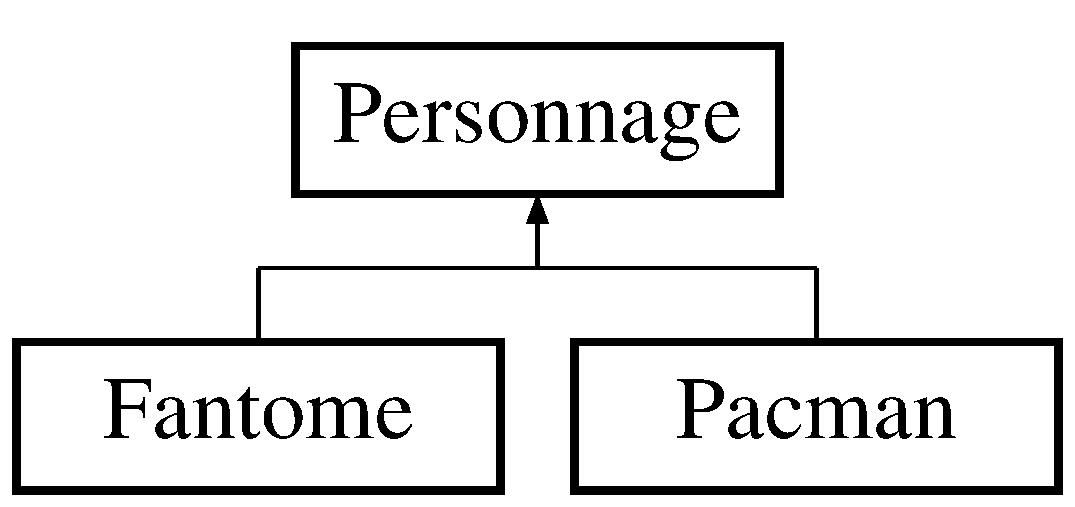
\includegraphics[height=2.000000cm]{class_personnage}
\end{center}
\end{figure}
\subsection*{Public Types}
\begin{DoxyCompactItemize}
\item 
\hypertarget{class_personnage_a4fd878262e17985fe2c4d59b5d816bd5}{}enum {\bfseries direction} \{ \\*
{\bfseries right}, 
{\bfseries left}, 
{\bfseries up}, 
{\bfseries down}, 
\\*
{\bfseries none}
 \}\label{class_personnage_a4fd878262e17985fe2c4d59b5d816bd5}

\end{DoxyCompactItemize}
\subsection*{Public Member Functions}
\begin{DoxyCompactItemize}
\item 
\hyperlink{class_personnage_ac0d494004d7fc8aac08112ff5ffacfe9}{Personnage} (float x, float y)
\begin{DoxyCompactList}\small\item\em Personnage\+::\+Personnage constructeur avec paramètre de personnage. \end{DoxyCompactList}\item 
float \hyperlink{class_personnage_a27cc1b2cd8f95546b646d5693157b3c6}{getx} ()
\begin{DoxyCompactList}\small\item\em \hyperlink{class_personnage_a27cc1b2cd8f95546b646d5693157b3c6}{Personnage\+::getx}. \end{DoxyCompactList}\item 
float \hyperlink{class_personnage_acaa6215bf06086ebf688e2b2e2e676f5}{gety} ()
\begin{DoxyCompactList}\small\item\em \hyperlink{class_personnage_acaa6215bf06086ebf688e2b2e2e676f5}{Personnage\+::gety}. \end{DoxyCompactList}\item 
int \hyperlink{class_personnage_aac0bd2c4c3bda5d26af8060f348e2b38}{getw} ()
\begin{DoxyCompactList}\small\item\em \hyperlink{class_personnage_aac0bd2c4c3bda5d26af8060f348e2b38}{Personnage\+::getw}. \end{DoxyCompactList}\item 
int \hyperlink{class_personnage_a29d38db07c8e6406caeea2fa832374af}{geth} ()
\begin{DoxyCompactList}\small\item\em \hyperlink{class_personnage_a29d38db07c8e6406caeea2fa832374af}{Personnage\+::geth}. \end{DoxyCompactList}\item 
direction \hyperlink{class_personnage_afff305624380f7fea61ea34d25a23db0}{getdir} ()
\begin{DoxyCompactList}\small\item\em \hyperlink{class_personnage_afff305624380f7fea61ea34d25a23db0}{Personnage\+::getdir}. \end{DoxyCompactList}\item 
void \hyperlink{class_personnage_a017efb88daf72424a7b1e23431bcf60f}{setx} (float x)
\begin{DoxyCompactList}\small\item\em \hyperlink{class_personnage_a017efb88daf72424a7b1e23431bcf60f}{Personnage\+::setx} modifie la position horizontale. \end{DoxyCompactList}\item 
void \hyperlink{class_personnage_ac91b7c71a7f25e3e1696469e7012383d}{sety} (float y)
\begin{DoxyCompactList}\small\item\em \hyperlink{class_personnage_ac91b7c71a7f25e3e1696469e7012383d}{Personnage\+::sety} modifie la position verticale. \end{DoxyCompactList}\item 
void \hyperlink{class_personnage_adb1c763969fee6521f870a21b2593387}{setw} (int w)
\begin{DoxyCompactList}\small\item\em \hyperlink{class_personnage_adb1c763969fee6521f870a21b2593387}{Personnage\+::setw} modifie la largeur. \end{DoxyCompactList}\item 
void \hyperlink{class_personnage_a27cec3441dcb29cdd98aceb107e0a6d4}{seth} (int h)
\begin{DoxyCompactList}\small\item\em \hyperlink{class_personnage_a27cec3441dcb29cdd98aceb107e0a6d4}{Personnage\+::seth} modifie hauteur. \end{DoxyCompactList}\item 
void \hyperlink{class_personnage_a4f68109b5502cf8dd451cfde07ea0f80}{setdir} (direction dir)
\begin{DoxyCompactList}\small\item\em \hyperlink{class_personnage_a4f68109b5502cf8dd451cfde07ea0f80}{Personnage\+::setdir} change la direction. \end{DoxyCompactList}\item 
\hypertarget{class_personnage_aa0e21a766208ea65c9929a8121e18dbe}{}Q\+Graphics\+Pixmap\+Item $\ast$ {\bfseries getgobj} ()\label{class_personnage_aa0e21a766208ea65c9929a8121e18dbe}

\item 
\hypertarget{class_personnage_a99c5442355ae6ebd56f34055a114ba69}{}void \hyperlink{class_personnage_a99c5442355ae6ebd56f34055a114ba69}{reinit} ()\label{class_personnage_a99c5442355ae6ebd56f34055a114ba69}

\begin{DoxyCompactList}\small\item\em \hyperlink{class_personnage_a99c5442355ae6ebd56f34055a114ba69}{Personnage\+::reinit}. \end{DoxyCompactList}\item 
void \hyperlink{class_personnage_a6ae5430d11fd2f01a4219722d860929f}{move} (\hyperlink{class_labyrinthe}{Labyrinthe} $\ast$l)
\begin{DoxyCompactList}\small\item\em \hyperlink{class_personnage_a6ae5430d11fd2f01a4219722d860929f}{Personnage\+::move} gère le déplacement d\textquotesingle{}un personnage dans le labyrinthe. \end{DoxyCompactList}\item 
\hypertarget{class_personnage_a5791bfb8523c996039f4376c7daf4881}{}void \hyperlink{class_personnage_a5791bfb8523c996039f4376c7daf4881}{Collision\+Lab} ()\label{class_personnage_a5791bfb8523c996039f4376c7daf4881}

\begin{DoxyCompactList}\small\item\em \hyperlink{class_personnage_a5791bfb8523c996039f4376c7daf4881}{Personnage\+::\+Collision\+Lab} gestion de la position du personnage en cas de collision avec un mur du labyrinthe. \end{DoxyCompactList}\item 
\hypertarget{class_personnage_a97bb68a40dc43e1c4a0ac920fb24e4ad}{}virtual \hyperlink{class_personnage}{Personnage} $\ast$ {\bfseries resize} (int w, int h)\label{class_personnage_a97bb68a40dc43e1c4a0ac920fb24e4ad}

\end{DoxyCompactItemize}
\subsection*{Protected Attributes}
\begin{DoxyCompactItemize}
\item 
\hypertarget{class_personnage_a6b996f03f323c2c74c5087ea69845a12}{}Q\+Graphics\+Pixmap\+Item $\ast$ {\bfseries gobj}\label{class_personnage_a6b996f03f323c2c74c5087ea69845a12}

\item 
\hypertarget{class_personnage_ad69bcd59258593fb200adb0e86bd7e9b}{}float {\bfseries x}\label{class_personnage_ad69bcd59258593fb200adb0e86bd7e9b}

\item 
\hypertarget{class_personnage_a3827e0cf147db7cc31e3967b23c4395d}{}float {\bfseries y}\label{class_personnage_a3827e0cf147db7cc31e3967b23c4395d}

\item 
\hypertarget{class_personnage_ab246d91c6787ccd5cec5664f7e5d478a}{}int {\bfseries w}\label{class_personnage_ab246d91c6787ccd5cec5664f7e5d478a}

\item 
\hypertarget{class_personnage_a5dd35ace58df8299a92fddee390e1e55}{}int {\bfseries h}\label{class_personnage_a5dd35ace58df8299a92fddee390e1e55}

\item 
\hypertarget{class_personnage_a9ea72b045c379d8fa5938fcb7129ace2}{}int {\bfseries offset}\label{class_personnage_a9ea72b045c379d8fa5938fcb7129ace2}

\item 
\hypertarget{class_personnage_a7a74d1843f448cb007e5c4db909f9bac}{}int {\bfseries initx}\label{class_personnage_a7a74d1843f448cb007e5c4db909f9bac}

\item 
\hypertarget{class_personnage_ac94d042476be54e7a84446a35aaa82e1}{}int {\bfseries inity}\label{class_personnage_ac94d042476be54e7a84446a35aaa82e1}

\item 
\hypertarget{class_personnage_a03d309b13ca5e26fcc04dca85378baf8}{}direction {\bfseries dir}\label{class_personnage_a03d309b13ca5e26fcc04dca85378baf8}

\end{DoxyCompactItemize}


\subsection{Constructor \& Destructor Documentation}
\hypertarget{class_personnage_ac0d494004d7fc8aac08112ff5ffacfe9}{}\index{Personnage@{Personnage}!Personnage@{Personnage}}
\index{Personnage@{Personnage}!Personnage@{Personnage}}
\subsubsection[{Personnage(float x, float y)}]{\setlength{\rightskip}{0pt plus 5cm}Personnage\+::\+Personnage (
\begin{DoxyParamCaption}
\item[{float}]{x, }
\item[{float}]{y}
\end{DoxyParamCaption}
)}\label{class_personnage_ac0d494004d7fc8aac08112ff5ffacfe9}


Personnage\+::\+Personnage constructeur avec paramètre de personnage. 


\begin{DoxyParams}{Parameters}
{\em x} & position horizontale \\
\hline
{\em y} & position verticale \\
\hline
\end{DoxyParams}


\subsection{Member Function Documentation}
\hypertarget{class_personnage_afff305624380f7fea61ea34d25a23db0}{}\index{Personnage@{Personnage}!getdir@{getdir}}
\index{getdir@{getdir}!Personnage@{Personnage}}
\subsubsection[{getdir()}]{\setlength{\rightskip}{0pt plus 5cm}Personnage\+::direction Personnage\+::getdir (
\begin{DoxyParamCaption}
{}
\end{DoxyParamCaption}
)}\label{class_personnage_afff305624380f7fea61ea34d25a23db0}


\hyperlink{class_personnage_afff305624380f7fea61ea34d25a23db0}{Personnage\+::getdir}. 

\begin{DoxyReturn}{Returns}
direction 
\end{DoxyReturn}
\hypertarget{class_personnage_a29d38db07c8e6406caeea2fa832374af}{}\index{Personnage@{Personnage}!geth@{geth}}
\index{geth@{geth}!Personnage@{Personnage}}
\subsubsection[{geth()}]{\setlength{\rightskip}{0pt plus 5cm}int Personnage\+::geth (
\begin{DoxyParamCaption}
{}
\end{DoxyParamCaption}
)}\label{class_personnage_a29d38db07c8e6406caeea2fa832374af}


\hyperlink{class_personnage_a29d38db07c8e6406caeea2fa832374af}{Personnage\+::geth}. 

\begin{DoxyReturn}{Returns}
hauteur 
\end{DoxyReturn}
\hypertarget{class_personnage_aac0bd2c4c3bda5d26af8060f348e2b38}{}\index{Personnage@{Personnage}!getw@{getw}}
\index{getw@{getw}!Personnage@{Personnage}}
\subsubsection[{getw()}]{\setlength{\rightskip}{0pt plus 5cm}int Personnage\+::getw (
\begin{DoxyParamCaption}
{}
\end{DoxyParamCaption}
)}\label{class_personnage_aac0bd2c4c3bda5d26af8060f348e2b38}


\hyperlink{class_personnage_aac0bd2c4c3bda5d26af8060f348e2b38}{Personnage\+::getw}. 

\begin{DoxyReturn}{Returns}
largeur 
\end{DoxyReturn}
\hypertarget{class_personnage_a27cc1b2cd8f95546b646d5693157b3c6}{}\index{Personnage@{Personnage}!getx@{getx}}
\index{getx@{getx}!Personnage@{Personnage}}
\subsubsection[{getx()}]{\setlength{\rightskip}{0pt plus 5cm}float Personnage\+::getx (
\begin{DoxyParamCaption}
{}
\end{DoxyParamCaption}
)}\label{class_personnage_a27cc1b2cd8f95546b646d5693157b3c6}


\hyperlink{class_personnage_a27cc1b2cd8f95546b646d5693157b3c6}{Personnage\+::getx}. 

\begin{DoxyReturn}{Returns}
position horizontale 
\end{DoxyReturn}
\hypertarget{class_personnage_acaa6215bf06086ebf688e2b2e2e676f5}{}\index{Personnage@{Personnage}!gety@{gety}}
\index{gety@{gety}!Personnage@{Personnage}}
\subsubsection[{gety()}]{\setlength{\rightskip}{0pt plus 5cm}float Personnage\+::gety (
\begin{DoxyParamCaption}
{}
\end{DoxyParamCaption}
)}\label{class_personnage_acaa6215bf06086ebf688e2b2e2e676f5}


\hyperlink{class_personnage_acaa6215bf06086ebf688e2b2e2e676f5}{Personnage\+::gety}. 

\begin{DoxyReturn}{Returns}
position verticale 
\end{DoxyReturn}
\hypertarget{class_personnage_a6ae5430d11fd2f01a4219722d860929f}{}\index{Personnage@{Personnage}!move@{move}}
\index{move@{move}!Personnage@{Personnage}}
\subsubsection[{move(\+Labyrinthe $\ast$l)}]{\setlength{\rightskip}{0pt plus 5cm}void Personnage\+::move (
\begin{DoxyParamCaption}
\item[{{\bf Labyrinthe} $\ast$}]{l}
\end{DoxyParamCaption}
)}\label{class_personnage_a6ae5430d11fd2f01a4219722d860929f}


\hyperlink{class_personnage_a6ae5430d11fd2f01a4219722d860929f}{Personnage\+::move} gère le déplacement d\textquotesingle{}un personnage dans le labyrinthe. 


\begin{DoxyParams}{Parameters}
{\em l} & pointeur vers le labyrinthe \\
\hline
\end{DoxyParams}
\hypertarget{class_personnage_a4f68109b5502cf8dd451cfde07ea0f80}{}\index{Personnage@{Personnage}!setdir@{setdir}}
\index{setdir@{setdir}!Personnage@{Personnage}}
\subsubsection[{setdir(direction dir)}]{\setlength{\rightskip}{0pt plus 5cm}void Personnage\+::setdir (
\begin{DoxyParamCaption}
\item[{direction}]{dir}
\end{DoxyParamCaption}
)}\label{class_personnage_a4f68109b5502cf8dd451cfde07ea0f80}


\hyperlink{class_personnage_a4f68109b5502cf8dd451cfde07ea0f80}{Personnage\+::setdir} change la direction. 


\begin{DoxyParams}{Parameters}
{\em dir} & nouvelle direction \\
\hline
\end{DoxyParams}
\hypertarget{class_personnage_a27cec3441dcb29cdd98aceb107e0a6d4}{}\index{Personnage@{Personnage}!seth@{seth}}
\index{seth@{seth}!Personnage@{Personnage}}
\subsubsection[{seth(int h)}]{\setlength{\rightskip}{0pt plus 5cm}void Personnage\+::seth (
\begin{DoxyParamCaption}
\item[{int}]{h}
\end{DoxyParamCaption}
)}\label{class_personnage_a27cec3441dcb29cdd98aceb107e0a6d4}


\hyperlink{class_personnage_a27cec3441dcb29cdd98aceb107e0a6d4}{Personnage\+::seth} modifie hauteur. 


\begin{DoxyParams}{Parameters}
{\em h} & hauteur \\
\hline
\end{DoxyParams}
\hypertarget{class_personnage_adb1c763969fee6521f870a21b2593387}{}\index{Personnage@{Personnage}!setw@{setw}}
\index{setw@{setw}!Personnage@{Personnage}}
\subsubsection[{setw(int w)}]{\setlength{\rightskip}{0pt plus 5cm}void Personnage\+::setw (
\begin{DoxyParamCaption}
\item[{int}]{w}
\end{DoxyParamCaption}
)}\label{class_personnage_adb1c763969fee6521f870a21b2593387}


\hyperlink{class_personnage_adb1c763969fee6521f870a21b2593387}{Personnage\+::setw} modifie la largeur. 


\begin{DoxyParams}{Parameters}
{\em w} & largeur \\
\hline
\end{DoxyParams}
\hypertarget{class_personnage_a017efb88daf72424a7b1e23431bcf60f}{}\index{Personnage@{Personnage}!setx@{setx}}
\index{setx@{setx}!Personnage@{Personnage}}
\subsubsection[{setx(float x)}]{\setlength{\rightskip}{0pt plus 5cm}void Personnage\+::setx (
\begin{DoxyParamCaption}
\item[{float}]{x}
\end{DoxyParamCaption}
)}\label{class_personnage_a017efb88daf72424a7b1e23431bcf60f}


\hyperlink{class_personnage_a017efb88daf72424a7b1e23431bcf60f}{Personnage\+::setx} modifie la position horizontale. 


\begin{DoxyParams}{Parameters}
{\em x} & nouvelle position horizontale \\
\hline
\end{DoxyParams}
\hypertarget{class_personnage_ac91b7c71a7f25e3e1696469e7012383d}{}\index{Personnage@{Personnage}!sety@{sety}}
\index{sety@{sety}!Personnage@{Personnage}}
\subsubsection[{sety(float y)}]{\setlength{\rightskip}{0pt plus 5cm}void Personnage\+::sety (
\begin{DoxyParamCaption}
\item[{float}]{y}
\end{DoxyParamCaption}
)}\label{class_personnage_ac91b7c71a7f25e3e1696469e7012383d}


\hyperlink{class_personnage_ac91b7c71a7f25e3e1696469e7012383d}{Personnage\+::sety} modifie la position verticale. 


\begin{DoxyParams}{Parameters}
{\em y} & nouvelle position verticale \\
\hline
\end{DoxyParams}


The documentation for this class was generated from the following files\+:\begin{DoxyCompactItemize}
\item 
C\+:/\+Users/kelku/\+Documents/\+Git\+Hub/pac/\+Pacman/personnage.\+h\item 
C\+:/\+Users/kelku/\+Documents/\+Git\+Hub/pac/\+Pacman/personnage.\+cpp\end{DoxyCompactItemize}

%--- End generated contents ---

% Index
\backmatter
\newpage
\phantomsection
\clearemptydoublepage
\addcontentsline{toc}{chapter}{Index}
\printindex

\end{document}
